\section{Heapsort}
O algoritmo Heapsort foi introduzido por J. W. J. Williams em 1964, no artigo \textit{Algorithm 232: Heapsort}, publicado na revista \textit{Communications of the ACM}. Como o próprio nome sugere, este algoritmo faz uso de uma estrutura de dados chamada \textit{heap}, mais especificamente um \textit{max-heap} binário.

\subsection*{\textit{max-heap} binário}
Um \textit{max-heap} binário -- de agora em diante referido apenas como \textit{heap} -- é uma árvore binária quase completa que satisfaz a propriedade de que o valor armazenado em um nó pai é maior ou igual ao valor de seus filhos. Uma árvore binária é considerada quase completa quando todos os seus níveis estão completamente preenchidos, exceto possivelmente o último, que deve ser preenchido da esquerda para a direita.

Convenientemente, essa árvore pode ser implementada em um vetor, de modo que cada posição do vetor represente um nó da árvore. Os filhos do nó na posição $i$ estão localizados nas posições $2i + 1$ e $2i + 2$, desde que essas posições sejam válidas.

\begin{figure}[H]
\Caption{\label{fig:maxheap}Exemplo de max-heap binário.}
\centering
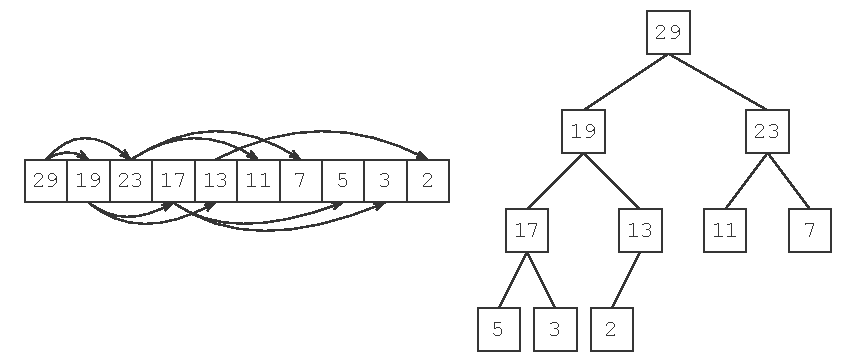
\includegraphics[scale=1.0]{figuras/pdf/max-heap.pdf}
\Fonte{Elaborado pelo autor.}
\end{figure}

\subsection*{Função Heapifica}
A função Heapifica será usada tanto para construir o \textit{heap} quanto para implementar o Heapsort em si. Ela é responsável por restaurar a propriedade de \textit{heap} em um ``quase \textit{heap}''. Um ``quase \textit{heap}'' é uma árvore em que apenas a raiz pode estar violando a propriedade de \textit{heap}. A ideia é simples: começando pela raiz, compara-se o nó atual com seu filho de maior valor; se o filho for maior, os dois são trocados de posição, e o processo é repetido com o novo nó até que a condição seja falsa ou uma folha seja atingida.
\lstinputlisting[language=C]{codigos/aux/heapifica.txt}

\subsection*{Construção do heap}
Considere o problema de transformar um vetor em um \textit{heap}. Para resolvê-lo, basta aplicar a operação Heapifica a todos os nós que não são folhas, da direita para a esquerda.
\lstinputlisting[language=C]{codigos/aux/constroi_heap.txt}

\subsection*{O algoritmo Heapsort}
O Heapsort começa transformando o vetor de entrada em um \textit{heap}. Após isso, o maior elemento estará na primeira posição. Sabendo disso, $v[0]$ é trocado com $v[n - 1]$. Neste momento, o maior elemento está na posição correta, e $v[0..n - 2]$ forma um “quase \textit{heap}”. Em seguida, a função Heapifica transforma $v[0..n - 2]$ em um \textit{heap}, e esse processo é repetido até que o \textit{heap} tenha apenas um elemento.
\lstinputlisting[language=C]{codigos/sup/3_heapsort.txt}

\subsection*{Desempenho}
A quantidade de operações que a função Heapifica executa quando invocada em um nó de altura $h$ é proporcional a $h$. Além disso, existem exatamente $2^M / 2^h$ nós com altura $h > 1$, onde $M = \lfloor \log_2 n \rfloor + 1$. Logo, a quantidade total de operações na construção do \textit{heap} é dada por:
\[
\sum_{h=2}^{M} h\left(\frac{2^M}{2^h}\right) \;=\; 2^M\cdot\sum_{h=2}^{M} h\left(\frac{1}{2}\right)^h \;\;<\;\; 2^M\cdot\sum_{h=1}^{\infty} h\left(\frac{1}{2}\right)^h \;=\; 2^{M+1} \;\;\approx\;\; 2n
\]
Portanto, o \textit{heap} é construído em tempo linear, \bigO{n}. Já a segunda parte do algoritmo, a partir da linha 3, executa aproximadamente
\[
\sum_{i=1}^{n-1} \log_2 i \;=\; \log_2 (n-1)! \;\;\leq\;\; n\log_2 n
\]
operações e, portanto, todo o algoritmo consome tempo proporcional a \bigO{n\log_2 n}.
